% 初中衔接：圆心 O(0,0)、半径3、P(5,0)，真实切点 A(9/5,12/5), B(9/5,-12/5)
\begin{center}
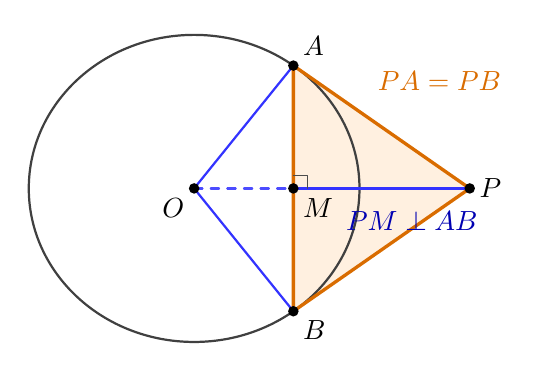
\begin{tikzpicture}[x=0.70cm,y=0.65cm,line cap=round,line join=round]
  \coordinate (O) at (0,0);
  \coordinate (P) at (5,0);
  \coordinate (A) at (1.8,2.4);
  \coordinate (B) at (1.8,-2.4);
  \coordinate (M) at (1.8,0);
  \fill[orange!12] (P)--(A)--(B)--cycle;
  \draw[thick,black!75] (O) circle (3);
  \draw[very thick,orange!85!black] (P)--(A)--(B)--cycle;
  \draw[blue!80,thick] (O)--(A) (O)--(B);
  \draw[blue!70,dashed,thick] (O)--(P);
  \draw[blue!80,very thick] (P)--(M);
  % Since AB is vertical and PM horizontal, their crossing is perpendicular.
  \draw[thin,black!70] (1.8,0.25)--(2.05,0.25)--(2.05,0);
  \fill (O) circle (1.9pt) node[below left] {$O$};
  \fill (P) circle (1.9pt) node[right] {$P$};
  \fill (A) circle (1.9pt) node[above right] {$A$};
  \fill (B) circle (1.9pt) node[below right] {$B$};
  \fill (M) circle (1.9pt) node[below right] {$M$};
  \node[orange!85!black] at (4.45,2.1) {$PA=PB$};
  \node[blue!70!black] at (3.95,-0.63) {$PM\perp AB$};
\end{tikzpicture}
\end{center}
